%%%%%%%%%%%%%%%%%%%%%
% Likelihood stuff
%%%%%%%%%%%%%%%%%%%%%


The razor boost analysis defines one signal region and three control regions, all of which are
divided into 25 bins on the ($\mr$,$\rsq$) space. The control regions are used to constrain the
background in the signal region.
The structure of the probability model, which comprises a likelihood for the signal
region and an evidence based prior for the background components, is illustrated in
Fig.~\ref{fig:boost_flowchart}. 

The expected background contributions in the signal region $S$, represented by the blue circle in
the figure, are denoted by $b^S_{\rm process}$. The index representing the ($\mr$,$\rsq$) bin has
been suppressed in this notation. It is important to remember, however, that the background
estimation is done bin-by-bin.  
The three main background components, $b^S_{\rm QCD}$, $b^S_{t\bar{t}+t}$, and $b^S_{\W\ell\nu}$,
are constrained by data in the three control regions, $Q$, $T$, and $W$, respectively. 
The expected background count $b_{\rm oth}^S$ comprises all the other, smaller, background
processes, and is constrained using MC simulated data. 

The control regions are shown in the green, red, and magenta circles in
Fig.~\ref{fig:boost_flowchart}. The connections between the different circles indicate the
relations between the signal and control regions. These relations are encapsulated in the global
translation factors $\kappa^{A/B}_{\rm process}$, where $A$ and $B$ represent any two regions. 
Consider the $W$ region as example, where we see a link between the $W$ and $S$ region. This link
exists because we use the $W$ region to constrain the $\W(\rightarrow \ell\nu)+$jets background in
the signal region, $b^S_{\W\ell\nu}$. The way this is done is by relating the $\W(\rightarrow
\ell\nu)+$jets contribution in both regions via the scale factor $\kappa^{W/S}_{\W\ell\nu}$, 
\begin{equation}
  b^W_{\W\ell\nu} = \kappa^{W/S}_{\W\ell\nu} b^S_{\W\ell\nu}  .
\end{equation}
The total expected count in the $W$ region is just a sum over the components listed within the
coloured circle, 
\begin{equation}
  b^W_{\rm total} = \kappa^{W/S}_{\W\ell\nu} b^S_{\W\ell\nu}  + b_{\rm oth}^W .
\end{equation}
The count for the small other components, $b_{\rm oth}^W$, is again constrained using simulation.
The observed data count in the $W$ region will be denoted by $N^W$. 
As mentioned several times before, the scale factors $\kappa$ are global scale factors, meaning that
they are not computed separately for each ($\mr$,$\rsq$) bin, but rather integrated across all 25
bins. For the example of the $W$ region this becomes,
\begin{equation}
  \kappa^{W/S}_{\W\ell\nu} = \frac{ \sum_{i=1}^{25} b^W_{\W\ell\nu, {\rm MC}, i}} {
\sum_{i=1}^{25} b^S_{\W\ell\nu, {\rm MC}, i}} ,
\label{eq:kappa_example}
\end{equation}
where we have added the subscript MC to indicate that MC simulation is used to determine these
counts. 
The total expected counts in the $T$ and $Q$ regions can be computed in a similar fashion, as a sum
of the contributions listed in the respective coloured circles in the figure. For the $T$ region
there is a small complication because we also use the $Q$ region to constrain the multijet
background in the $T$ region. 

\begin{figure}[p]
  \centering
  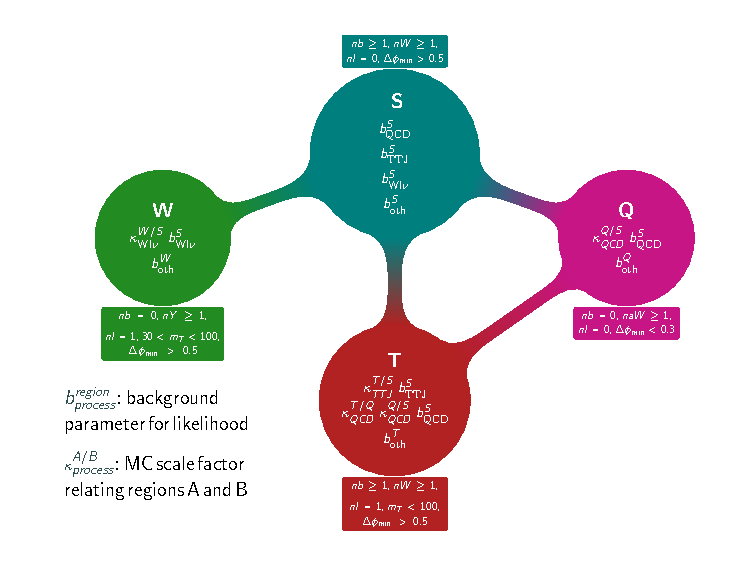
\includegraphics[width=\textwidth]{figures/razor_strategy/BoostFlowChart_noZ}
  \caption{Definition of, and relationship between, the signal ($S$) and control ($Q,T,W$) regions
and their relationship to the bin-by-bin background parameters
$b^{\textrm{region}}_{\textrm{process}}$ for a given region and background process, as well as the
four global scale factors $\kappa^{A/B}_{\textrm{process}} = \sum_i b^A_{\rm process, MC, i} /
\sum_i b^B_{\rm process, MC, i}$, where the sum is over all 25 (\mr,\rsq) bins of the simulated
data. 
The total expected background, per bin, is the sum of the terms shown for each region. Furthermore,
associated with each bin of each region is an observed count $N^{\textrm{region}}$, a simulated
count $N^{\textrm{region}}_{\rm process, MC}$, and a count $N^{\textrm{region}}_{\rm oth, MC}$
equal to the sum of the smaller backgrounds, with associated parameter
$b^{\textrm{region}}_{\rm oth}$.
  \label{fig:boost_flowchart}}
\end{figure}



The statistical analysis of the set of observations,  $\{ N^S_i \}$, in the signal region is based
on a likelihood function, $L(\sigma)$, given by
\begin{align}
  L(\sigma) & \equiv  \int   \left[ \prod_{i=1}^M p(N^S_i | \sigma, {\cal L}, \theta_i)  \right] 
\pi(\theta) \, \pi({\cal L}) \, d\theta \, d{\cal L},
\label{eq:marginal}
\end{align}
where $\sigma$ is the total signal cross section, and our parameter of interest.
The number of bins on the ($\mr$,$\rsq$) space is $M = 25$, $N^S_i$ is the observed count
in bin $i$, and the bin-by-bin parameters  $\epsilon$,  $b^S_{\rm QCD}, b^S_{t\bar{t}+t},
b^S_{\W\ell\nu}$, and $b^S_{\rm oth}$ are denoted collectively by $\theta$. 
The parameter $\epsilon$ represents the $M$ signal efficiencies (including acceptance) for a given
signal model. 
%
The function $\pi({\cal L})$ is the integrated luminosity prior and $\pi(\theta)$ is an evidence
based prior constructed from observations in the control regions and the four global scale factors
$\kappa^{A/B}_{\rm process}$ determined by simulated data. 
%
As mentioned, Fig.~\ref{fig:boost_flowchart} shows which control regions provide constraints on
each of the background parameters, $b^S_{\rm process}$.
%
The likelihood per ($\mr$,$\rsq$) bin is taken to be
\begin{equation}
 p(N^S | \sigma, {\cal L}, \theta) = \textrm{Poisson}(N^S,  \epsilon \sigma {\cal L} + b^S_{\rm QCD}
+ b^S_{t\bar{t}+t} + b^S_{\W\ell\nu} +  b^{S}_{\rm oth}) .
\end{equation}
The likelihood for all bins is then computed as a product of all per-bin likelihoods. 
It is clear from the left-hand side of Eq.~\ref{eq:marginal} that the final analysis likelihood only
depends on the signal cross section. The dependence on all other (nuisance) parameters has been
removed through marginalization. 

The integral in Eq.~(\ref{eq:marginal}) is approximated by Monte Carlo integration by sampling
the priors $\pi({\cal L})$ and  $\pi(\theta)$, 
\begin{equation}
    L(\sigma) \approx \frac{1}{J} \sum_{j=1}^J \prod_{i=1}^{M}
    p(N^S_i| \sigma, \mathcal{L}_j, \theta_j),
\end{equation}
using $J$ points $\theta_j$ randomly sampled from the priors.
The priors for the expected integrated luminosity ${\cal L}$, signal efficiencies $\epsilon$, and 
simulated background counts $b^{\rm region}_{\rm process, MC}$ (which enter the computation of the
$\kappa$ factors), are modelled with gamma densities,
\begin{align}
\textrm{gamma}(x, \gamma, \beta) &= \beta^{-1}(x/\beta)^{\gamma-1} \exp(-x / \beta) /
\Gamma(\gamma),
\label{eq:gamma}
\end{align}
in which the mode is set to $c$ and the variance to $\delta c^2$, 
where $c \pm \delta c$ denotes either the measured integrated luminosity, or for a given bin of
a given region and process, the simulated signal efficiency, or the simulated background count. This
yields the gamma density parameters,
\begin{align}
   \gamma &= [(k + 2) + \sqrt{(k+2)^2 - 4}]/2,\\
   \beta &= [\sqrt{c^2 + 4\delta c^2} - c]/2,
\end{align}
where $k = (c / \delta c)^2$.
For empty bins, we set $\gamma = 1$ and the bin value is constrained to zero by setting the $\beta$
parameter to $10^{-4}$.

The prior for the expected signal efficiencies and background counts, $\pi(\theta)$, 
includes the uncertainties coming from the various systematic effects, which will be described in
more detail in Section~\ref{sec:boost_systematics}. 
The prior is modelled hierarchically, 
\begin{align}
  \pi(\theta) = \int \pi(\theta | c ) \, \pi(c | \phi ) \pi(\phi) \, dc d\phi,
  \label{eq:prior}
\end{align}
where $c$ is a simulated count or efficiency in an ($\mr$,$\rsq$) bin and $\phi$ represents
parameters that characterize the independent sources of systematic uncertainty. 
The integral in Eq.~(\ref{eq:prior}) is evaluated via MC integration in the following way.

First, $\phi$ values are sampled from $\pi(\phi)$, by drawing random numbers from a Gaussian
variate.
Then, $c$ values are sampled from $\pi(c | \phi)$, followed by $\theta$ values from $\pi(\theta |
c)$. 
The sampling from $\pi(\theta|c)$ is straightforward because the functional form is known.
For the simulated counts and efficiencies the afore-mentioned gamma densities are used, while the
observed counts in the control regions are modelled with Poisson densities.
%
However, $\pi(c | \phi)$ has an unknown shape, and the sampling of $c$ thus requires running the
analysis (in particular the event selection) multiple times, once for each sampling of the
systematic uncertainties. 
The novel feature of the razor boost analysis is that the independent sources of systematic
uncertainty are sampled simultaneously, and are then marginalized. This has the very
nice consequence that any correlations between systematic uncertainties, processes and
regions are properly taken into account. Practically, we produce an ensemble of sets of $(\mr,
\rsq)$ histograms for the simulated backgrounds and efficiencies, for all
signals under consideration, which automatically incorporate all statistical dependencies
without the need to model them explicitly. 

Once the ensemble of sets of ($\mr$,$\rsq$) histograms is produced, the sampling proceeds
as follows:
\begin{enumerate}
\item sample the integrated luminosity parameter;
\item sample the efficiency parameters, $\epsilon$, for every considered signal model;
\item sample the parameters $b^{\rm region}_{\rm process, MC}$ of the simulated background densities
and sum their values over the $M$ bins;
\item compute the $\kappa$ parameters from the appropriate background sums, for example as in
Eq.~\ref{eq:kappa_example};
\item scale $\kappa^{Q/S}_{\rm QCD}$ by a random Gaussian variate of unit mean and standard
deviation of 0.33 to account for additional uncertainty due to deficiencies in the
simulated data as determined from the second closure test (Section~\ref{sec:boost_closure_tests}),
resulting in a total uncertainty of 40\%;
\item sample the background parameters $b^S_{\rm QCD}$, $b^S_{t\bar{t}+t}$, and $b^S_{\W\ell\nu}$,
from the Poisson models  of the control regions; for example, for region $Q$, we map 
$\textrm{Poisson}(N^Q, \kappa^{Q/S}_{\rm QCD} b^S_{\rm QCD} + b^Q_{\rm oth})$ to a posterior density
in $b^S_{\rm QCD}$ using Bayes theorem and a flat prior and sample $b^S_{\rm QCD}$ from that
density.
\end{enumerate}
The expected background counts for each signal bin are then obtained from the sampled background
parameters, and are compared to the observations in data. The final results are shown in
Section~\ref{sec:boost_results}.

In the absence of  a signal, we determine limits on the total signal cross section using the CLs
criterion~\cite{LHCCLs} with the test statistic 
$t_\sigma = 2 \ln [ L(\hat{\sigma}) / L(\sigma)]$ when $0 \leq\hat{\sigma} \leq
\sigma$, 
and $t_\sigma = 0$ when $\hat{\sigma} > \sigma$. 
Large values of $t_\sigma$ indicate incompatibility between the best fit hypothesis 
$\sigma^\prime = \hat{\sigma}$ and the entertained hypothesis $\sigma^\prime  = \sigma$. 
We calculate the p-values 
\begin{equation}
p_0 = \textrm{Prob}(t_\sigma > t_{\sigma, obs} | \sigma^\prime = 0) ,
\end{equation}
and 
\begin{equation}
p_\sigma = \textrm{Prob}(t_\sigma > t_{\sigma, obs} | \sigma^\prime=\sigma) ,
\end{equation}
needed to calculate $\textrm{CLs}(\sigma) = p_\sigma / p_0$,  by simulation. 
The quantity $t_{\sigma, obs}$ denotes the observed values of the test statistic, one for each
hypothesis $\sigma^\prime=\sigma$.


